\documentclass[11pt,a4paper]{article}
\usepackage[margin=2.4cm]{geometry}
\usepackage[utf8]{inputenc}
\usepackage{microtype}
\usepackage{amsmath,amssymb,amsthm,mathtools,bm}
\usepackage{booktabs,array,enumitem,float,listings}
\usepackage[dvipsnames]{xcolor}
\usepackage{tikz,pgfplots}
\usetikzlibrary{arrows.meta,positioning,calc,shapes.geometric,patterns,fit,backgrounds}
\pgfplotsset{compat=1.16}
\usepackage[most]{tcolorbox}
\usepackage[hidelinks]{hyperref}

\lstset{basicstyle=\ttfamily\footnotesize,frame=single,backgroundcolor=\color{gray!6},
  language=Python,keywordstyle=\color{blue!60!black},commentstyle=\color{green!40!black},
  breaklines=true,columns=fullflexible,showstringspaces=false,xleftmargin=4pt,xrightmargin=4pt}

% ---------- macros ----------
\newcommand{\R}{\mathbb{R}}
\newcommand{\E}{\mathbb{E}}
\newcommand{\K}{\mathcal{K}}
\newcommand{\bx}{\bm{x}}
\newcommand{\bz}{\bm{z}}
\newcommand{\beps}{\bm{\epsilon}}
\newcommand{\slides}[1]{\texorpdfstring{\emph{(slides #1)}}{(slides #1)}}
\DeclareMathOperator*{\argmin}{arg\,min}

% ---------- theorem environments (amsthm) + boxes ----------
\theoremstyle{plain}
\newtheorem{theorem}{Theorem}[section]
\newtheorem{lemma}[theorem]{Lemma}
\newtheorem{proposition}[theorem]{Proposition}
\newtheorem{corollary}[theorem]{Corollary}
\theoremstyle{definition}
\newtheorem{definition}[theorem]{Definition}
\newtheorem{example}[theorem]{Example}
\newtheorem{algorithm}[theorem]{Algorithm}
\newtheorem{remark}[theorem]{Remark}
\numberwithin{equation}{section}

\tcbset{thmbox/.style={enhanced,breakable,boxrule=0.6pt,arc=2pt,left=6pt,right=6pt,top=4pt,bottom=4pt,before skip=8pt,after skip=8pt}}
\tcolorboxenvironment{definition}{thmbox,colframe=green!40!black,colback=green!3}
\tcolorboxenvironment{theorem}{thmbox,colframe=red!60!black,colback=red!3}
\tcolorboxenvironment{lemma}{thmbox,colframe=red!60!black,colback=red!3}
\tcolorboxenvironment{proposition}{thmbox,colframe=red!60!black,colback=red!3}
\tcolorboxenvironment{corollary}{thmbox,colframe=red!60!black,colback=red!3}
\tcolorboxenvironment{example}{thmbox,colframe=orange!80!black,colback=orange!4}
\tcolorboxenvironment{algorithm}{thmbox,colframe=violet!70!black,colback=violet!3}
\tcolorboxenvironment{remark}{thmbox,colframe=black!50,colback=black!3}

\newtcolorbox{intuition}{enhanced,breakable,colback=blue!5!white,colframe=blue!55!black,
  coltitle=white,fonttitle=\bfseries,title=Intuition,arc=2pt,boxrule=0.7pt,
  before skip=8pt,after skip=10pt,left=6pt,right=6pt}

% photo placeholder: \photo[height]{slide}{what to insert}
\newcommand{\photo}[3][2.8cm]{%
  \begin{center}\begin{tikzpicture}
  \node[draw,dashed,thick,fill=gray!8,minimum height=#1,text width=0.8\linewidth,align=center]
    {\textbf{[PHOTO PLACEHOLDER]}\\ Insert the image from \textbf{slide #2}:\\ \emph{#3}};
  \end{tikzpicture}\end{center}}

\tikzset{box/.style={draw,rounded corners=2pt,align=center,minimum height=0.8cm,fill=blue!8,inner sep=3pt,font=\small},
  frozen/.style={box,fill=pink!40},
  arr/.style={-{Stealth[length=2mm]},thick}}

\title{\textbf{Foundations of Spatial AI}\\[2pt] Lecture 03 --- Single-View Depth II\\[2pt]\large Detailed lecture notes}
\author{Notes on the slides of L.~Di Giammarino and E.~Giacomini (Sapienza University of Rome)}
\date{Lecture of September 30, 2026}

\begin{document}
\maketitle

\begin{abstract}\noindent
Part~I of the course obtained depth from a sensor (a laser, paid for in time) or from a network fitted to sensor labels (a prior, paid for in labels). Part~II, covered here, asks how far a prior can be pushed when labels are scarce or absent: (i) \emph{self-supervision} from stereo pairs, (ii) \emph{diffusion} as a generative prior, (iii) \emph{Marigold}, a depth estimator obtained by fine-tuning an image diffusion model, (iv) how affine errors distort the 3D reconstruction, and (v) \emph{Marigold-DC}, which steers the sampling loop with a few metric measurements. Section titles and their slide ranges follow the slide deck; slide numbers refer to the printed page numbers of the PDF.
\end{abstract}

\paragraph{About these notes.} Only the slide deck was provided (no companion book chapter). Formal statements are therefore taken from the slides themselves; where a proof or a derivation is not on the slides I supply it, and derivations that go beyond the slides are collected in Appendix~\ref{app:supp}. Blue \emph{Intuition} boxes explain the ideas in plain words. Photographs and rendered result images of the slides are replaced by dashed placeholders that say which slide to copy from; all conceptual diagrams are redrawn in TikZ.

\tableofcontents
\newpage

%=====================================================================
\section{Part I in One Slide \slides{1--2}}
%=====================================================================
Part~I obtained depth in two ways and closed \emph{owing two debts}:
\begin{itemize}[nosep]
  \item \textbf{Time.} A laser measures range directly: metric and exact where it lands, but sparse, and it produces the labels everything else trains on.
  \item \textbf{A prior.} A network fitted to those labels is dense and cheap, but it \emph{predicts} rather than recovers depth. The prior was fitted to labels that a sensor had to measure.
\end{itemize}
Mixing labels of different origin moved the output down a table, at a cost of free parameters.

\begin{definition}[Output types and their free parameters]
A depth-like output is defined only up to a transformation, and each transformation leaves free parameters that something else must later fix.
\begin{center}\small
\begin{tabular}{@{}lcl@{}}\toprule
output & free parameters & aligned by\\\midrule
metric depth & 0 & nothing\\
scale-invariant depth & 1 & one scale $s$\\
affine-invariant disparity or depth & 2 & scale and shift $(s,t)$\\
ordinal & any monotone map & nothing\\\bottomrule
\end{tabular}
\end{center}
\end{definition}

\begin{intuition}
Each free parameter is a \emph{number a sensor must still supply}. If a network says ``this pixel is twice as far as that one'', it has told you shape but not meters. Example: the truth is $D=2.0\,\hat D+0.3$~m. A metric network outputs $D$ itself; an affine-invariant one outputs $\hat D$ and you need the pair $(2.0,\,0.3)$ to recover meters. The whole lecture is about who supplies those numbers: the baseline of a stereo rig, a large generative prior, or a handful of LiDAR returns.
\end{intuition}

%=====================================================================
\section{Supervision without Ground Truth \slides{3--6}}
%=====================================================================
This is section 3.9 of the lecture. Its thesis: \emph{a stereo pair supplies its own supervision, provided the warp connecting the two images is differentiable.}

\subsection{View Synthesis and the Backward Warp \slides{4}}
Training uses stereo pairs $\{(\bm I_L,\bm I_R)\}$ only; there is no depth anywhere in the training set. The objective is to reproduce one image of the pair from the other. Depth is the only internal quantity that makes this task solvable, so if the network solves it, depth is what it must have learned. This holds only where a pixel is \textbf{textured} and visible in \textbf{both} views; elsewhere the objective says nothing and a hand-written prior fills the gap.

\begin{definition}[Backward warp]
Given a disparity map $d(u,v)$ defined on the \emph{target} image, the backward warp synthesizes the target from the source by
\begin{equation}
\tilde{\bm I}_L(u,v)=\bm I_R\bigl(u-d(u,v),\,v\bigr).
\end{equation}
Every \emph{target} pixel is mapped to exactly one \emph{source} location.
\end{definition}

\begin{proposition}[Why the warp must be backward]
Forward mapping (pushing each source pixel to a target location) lets several sources land on one target pixel and leaves other target pixels empty: collisions and holes. Backward mapping assigns each target pixel exactly one value, which makes the warp a \emph{differentiable function} of $d$ rather than a scatter operation.
\end{proposition}

\begin{figure}[H]
\centering
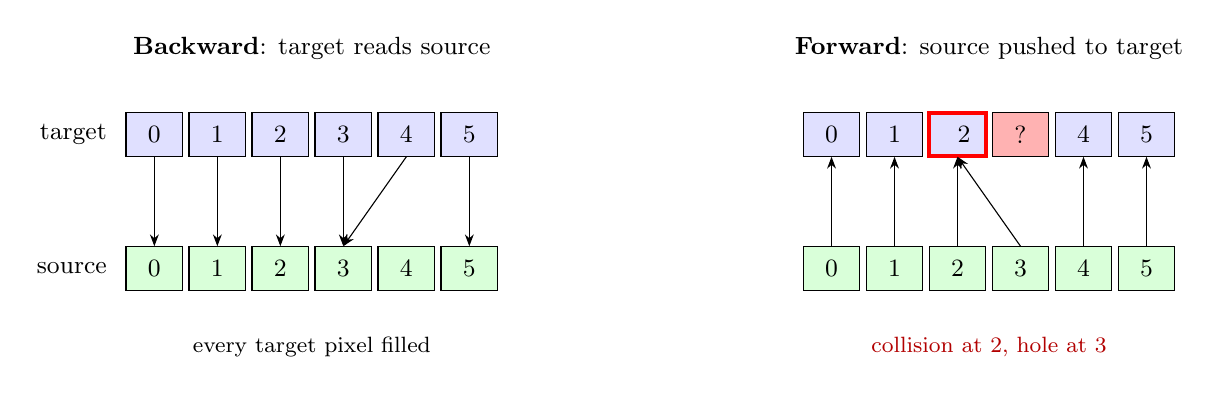
\begin{tikzpicture}[x=0.8cm,y=1cm,font=\small,
  pix/.style={draw,minimum width=0.72cm,minimum height=0.55cm,inner sep=0,fill=blue!12}]
\begin{scope}
 \node at (2.5,3.3) {\textbf{Backward}: target reads source};
 \foreach \i in {0,...,5}{\node[pix] (bt\i) at (\i,2.2){\i}; \node[pix,fill=green!15] (bs\i) at (\i,0.5){\i};}
 \node[anchor=east] at (-0.6,2.2){target}; \node[anchor=east] at (-0.6,0.5){source};
 \foreach \t/\s in {0/0,1/1,2/2,3/3,4/3,5/5}{\draw[-{Stealth[length=1.5mm]}] (bt\t.south)--(bs\s.north);}
 \node[font=\footnotesize,align=center] at (2.5,-0.5){every target pixel filled};
\end{scope}
\begin{scope}[xshift=8.6cm]
 \node at (2.5,3.3) {\textbf{Forward}: source pushed to target};
 \foreach \i in {0,...,5}{\node[pix] (ft\i) at (\i,2.2){\i}; \node[pix,fill=green!15] (fs\i) at (\i,0.5){\i};}
 \node[pix,fill=red!30] at (3,2.2){?};
 \node[pix,ultra thick,draw=red] at (2,2.2){\phantom{0}2};
 \foreach \s/\t in {0/0,1/1,2/2,3/2,4/4,5/5}{\draw[-{Stealth[length=1.5mm]}] (fs\s.north)--(ft\t.south);}
 \node[font=\footnotesize,align=center,text=red!70!black] at (2.5,-0.5){collision at 2, hole at 3};
\end{scope}
\end{tikzpicture}
\caption{Original 1D illustration of backward versus forward mapping (slide 4 shows the same effect on small coloured grids).}
\end{figure}

\begin{intuition}
Think of filling in a form versus mailing letters. Backward warping is the form: each target pixel asks \emph{``where in the other image should I look?''} and gets exactly one answer. Forward warping is the post office: every source pixel is mailed to an address; some mailboxes get two letters (collision), others none (hole), and ``two letters or none'' has no useful gradient. Note the sign convention: slide~4 writes $u-d$ for the left image as target, slide~5 writes $+d$ for a target/source pair set up the other way round; only the consistent use matters.
\end{intuition}

\subsection{Image Reconstruction as Supervision \slides{5}}
The pipeline of slide~5 has three steps: (1) a deep CNN predicts an inverse depth from the left image; (2) the right image is warped with it into a synthetic left image; (3) the reconstruction error against the real left image is the loss.

\begin{definition}[Disparity and photometric loss]
Under a rectified stereo rig with focal length $f$ and baseline $b$, the predicted inverse depth is the disparity
\begin{equation}
d(\bm p)=\frac{f\,b}{z(\bm p)}.
\end{equation}
The self-supervised loss compares the warped and real image,
\begin{equation}
\mathcal L_{\text{photo}}=\sum_{\bm p}\bigl\|\tilde{\bm I}(\bm p)-\bm I_L(\bm p)\bigr\|,\qquad \tilde{\bm I}(\bm p)=\bm I_R\bigl(\bm p+d(\bm p)\bigr).
\end{equation}
\end{definition}

\begin{figure}[H]
\centering
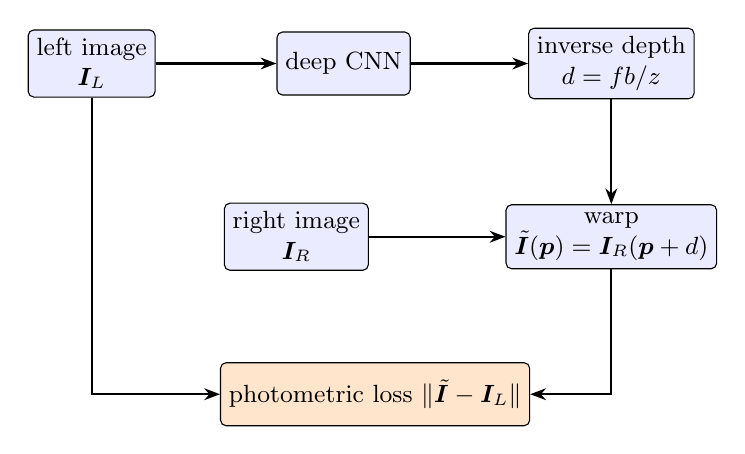
\begin{tikzpicture}[font=\small]
\node[box] (IL) at (0,0) {left image\\$\bm I_L$};
\node[box] (cnn) at (3.2,0) {deep CNN};
\node[box] (d) at (6.6,0) {inverse depth\\$d=fb/z$};
\node[box] (warp) at (6.6,-2.2) {warp\\$\tilde{\bm I}(\bm p)=\bm I_R(\bm p+d)$};
\node[box] (IR) at (2.6,-2.2) {right image\\$\bm I_R$};
\node[box,fill=orange!20] (loss) at (3.6,-4.2) {photometric loss $\|\tilde{\bm I}-\bm I_L\|$};
\draw[arr] (IL)--(cnn); \draw[arr] (cnn)--(d); \draw[arr] (d)--(warp);
\draw[arr] (IR)--(warp);
\draw[arr] (warp.south) |- (loss.east);
\draw[arr] (IL.south) |- (loss.west);
\end{tikzpicture}
\caption{Self-supervised stereo training (redrawn from slide 5). No depth label appears anywhere.}
\end{figure}

\photo[3cm]{5}{the KITTI street scene: left image, predicted inverse-depth map, warped image and reconstruction-error map (steps 1--3, with the red marker point)}

\begin{intuition}
Depth is the \emph{only} unknown the network can vary to make the warped image match the real one, so a network that solves the task has learned depth. Worked numbers (illustrative): with $f=700$~px and $b=0.5$~m, a car at $z=10$~m has $d=35$~px, whereas at $z=70$~m it has only $d=5$~px. Disparity is \emph{inverse} depth: distant objects move the image little, so the training signal is weak at range.
\end{intuition}

\subsection{Where the Loss Is Blind \slides{6}}
\begin{proposition}[Blind spots of the photometric loss]
(a) \emph{Textureless regions.} Writing the residual as $r=\bm I_R(u-d)-\bm I_L(u)$ and the squared loss as $\tfrac12 r^2$,
\begin{equation}
\frac{\partial \mathcal L}{\partial d}=-\,r\cdot \bm I_R'(u-d),
\end{equation}
which vanishes wherever $\bm I(u_0+1)\approx \bm I(u_0)$ (flat image, zero derivative): such pixels receive \emph{no training signal at all}.\\
(b) \emph{Occlusions.} A pixel visible to one camera only has no match in the other view, so the residual there is meaningless.
\end{proposition}

Both gaps are filled by hand-written priors: a smoothness term, left-right consistency, a minimum over the two reprojections, and masking of pixels that do not move between frames.

\begin{proposition}[The baseline decides what the trained model is worth]
Trained on a stereo pair, the model inherits the known baseline $b$ and is metric \emph{for that rig}. Trained on video, the baseline is unknown, so the output is shape up to one global scale and every image needs its own alignment.
\end{proposition}

\begin{intuition}
The photometric loss is a detective that only works with clues. Flat white wall: no clue, no gradient, so the smoothness prior guesses. Something hidden from one eye: no partner to compare with. The baseline is the ruler: with stereo the ruler length $b$ is known, so meters come free; with a monocular video the ruler length is not known, so you get a beautiful shape in unknown units (one free parameter, as in the table of Section~1).
\end{intuition}

%=====================================================================
\section{Diffusion, From Scratch \slides{7--22}}
%=====================================================================
This is section 3.10. Its thesis: \emph{a model trained to remove noise is a prior: it points toward the data from anywhere in the space, and it can be sampled, conditioned or steered.} (Adapted on the slides from MIT 6.S183, Lecture~1, by D.~Pfrommer.)

\subsection{Supervised Learning \slides{8}}
Supervised learning fits \textbf{one output per input}. At a depth edge that output is the average of the near surface and the far one: a distance that belongs to neither.

\begin{proposition}[MSE regression returns the conditional mean]
Let $Y$ be the target and $\bx$ the input. Among all functions $f$, the minimizer of $\E\|f(\bx)-Y\|^2$ is $f^\star(\bx)=\E[Y\mid\bx]$.
\end{proposition}
\begin{proof}
For fixed $\bx$ with $m=\E[Y\mid \bx]$, $\E[\|f-Y\|^2\mid\bx]=\|f-m\|^2+\E[\|Y-m\|^2\mid\bx]$; the second term does not depend on $f$, and the first is minimized by $f=m$.
\end{proof}

\begin{intuition}
At a depth edge half the training examples say $2$~m (near surface) and half say $10$~m (far surface). The best single answer under squared error is $6$~m, which is the depth of \emph{nothing}. That is the blurred, flying-pixel edge of regression networks.
\end{intuition}

\subsection{Generative Learning \slides{9}}
A generative model fits a \textbf{distribution} over outputs, not one value. ``The band is what a diffusion model represents.''

\begin{figure}[H]
\centering
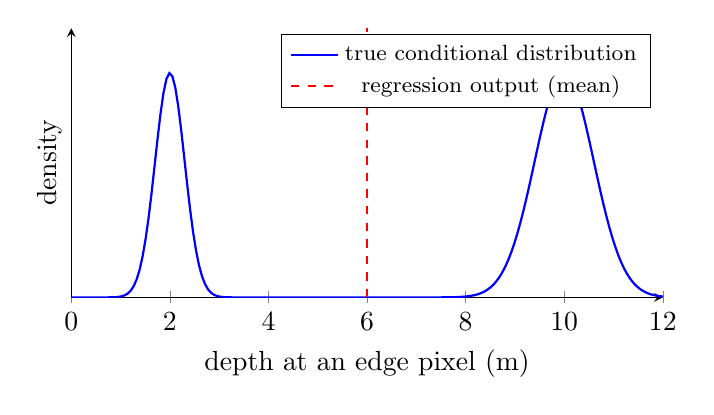
\begin{tikzpicture}
\begin{axis}[width=0.75\linewidth,height=5cm,domain=0:12,samples=200,axis lines=left,
  xlabel={depth at an edge pixel (m)},ylabel={density},ymajorticks=false,
  legend style={at={(0.98,0.98)},anchor=north east,font=\footnotesize}]
\addplot[thick,blue]{0.5*exp(-(x-2)^2/0.18)+0.5*exp(-(x-10)^2/0.72)};
\addplot[thick,red,dashed,samples=2] coordinates {(6,0)(6,0.6)};
\legend{true conditional distribution,regression output (mean)}
\end{axis}
\end{tikzpicture}
\caption{Original toy figure: a bimodal conditional distribution at a depth edge. The regressor answers the mean, which lies in a gap where the density is zero; a generative model can return a sample from one of the two modes.}
\end{figure}

\subsection{Many Outputs for One Input -- Text to Image \slides{10}}
One conditioning input has many valid completions. A regressor averages them; a diffusion model picks one.

\photo[3.6cm]{10}{left: grid of ``wearing\_glasses'' faces from regression (the mean face, blurred); right: grid of latent-diffusion samples (one sample, sharp)}

\begin{intuition}
Blur is not a training failure. It is the correct answer to the wrong question: the conditional mean of a set of sharp images is not a sharp image. The same averaging is what flattens a depth edge.
\end{intuition}

\subsection{The Forward and Reverse Process \slides{11}}
The \textbf{forward process} adds noise to data one step at a time until nothing of the data is left. It is fixed and has no parameters. It is inspired by Brownian motion (many small independent displacements), and after enough steps the sample is indistinguishable from Gaussian noise. A diffusion model learns the \textbf{reverse process}, which recovers data from noise; that reverse process \emph{is the prior}.

\begin{definition}[Forward and reverse processes]
The forward chain $q(\bx_t\mid\bx_{t-1})$ maps $\bx_0$ (data) to $\bx_T$ (noise) and is fixed; the model $p_\theta(\bx_{t-1}\mid\bx_t)$ learns the way back.
\end{definition}

\begin{figure}[H]
\centering
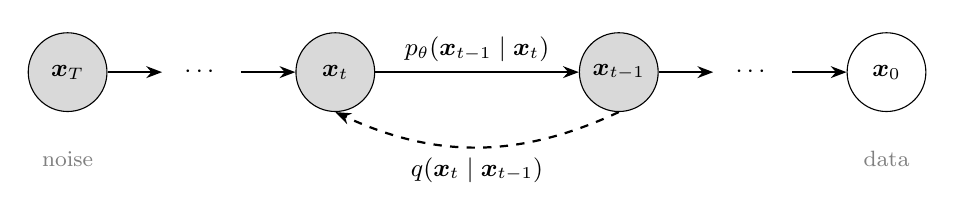
\begin{tikzpicture}[font=\small]
\node[draw,circle,fill=gray!30,minimum size=1cm] (xT) at (0,0){$\bx_T$};
\node at (1.7,0){$\cdots$};
\node[draw,circle,fill=gray!30,minimum size=1cm] (xt) at (3.4,0){$\bx_t$};
\node[draw,circle,fill=gray!30,minimum size=1cm] (xt1) at (7,0){$\bx_{t-1}$};
\node at (8.7,0){$\cdots$};
\node[draw,circle,minimum size=1cm] (x0) at (10.4,0){$\bx_0$};
\draw[arr] (xT)--(1.2,0); \draw[arr] (2.2,0)--(xt);
\draw[arr] (xt)--node[above]{$p_\theta(\bx_{t-1}\mid\bx_t)$}(xt1);
\draw[arr] (xt1)--(8.2,0); \draw[arr] (9.2,0)--(x0);
\draw[arr,dashed] (xt1.south) to[bend left=25] node[below]{$q(\bx_t\mid\bx_{t-1})$} (xt.south);
\node[font=\footnotesize,gray] at (0,-1.1){noise}; \node[font=\footnotesize,gray] at (10.4,-1.1){data};
\end{tikzpicture}
\caption{Forward (dashed, fixed) and reverse (solid, learned) chains, redrawn from slide 11.}
\end{figure}

\begin{figure}[H]
\centering
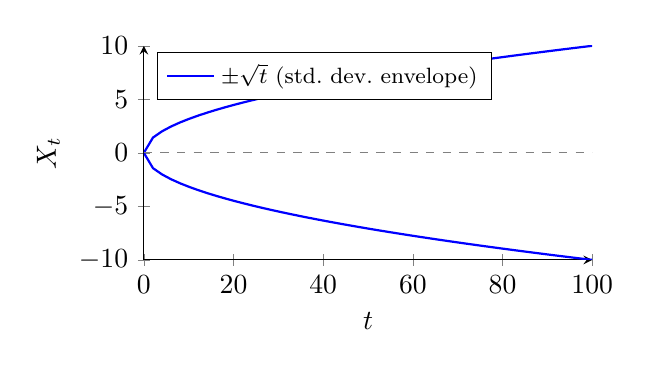
\begin{tikzpicture}
\begin{axis}[width=0.6\linewidth,height=4.3cm,domain=0:100,samples=50,axis lines=left,xlabel={$t$},ylabel={$X_t$},
  legend style={font=\footnotesize,at={(0.03,0.97)},anchor=north west}]
\addplot[thick,blue]{sqrt(x)}; \addplot[thick,blue]{-sqrt(x)}; \addplot[dashed,gray]{0};
\legend{$\pm\sqrt{t}$ (std.\ dev.\ envelope)}
\end{axis}
\end{tikzpicture}
\caption{Original figure: the spread of a random walk grows like $\sqrt t$, the mechanism that buries the data in noise.}
\end{figure}
\photo[3cm]{11}{Brownian-motion simulated paths (coloured bundle of trajectories) with the histogram of $X_T$ on the right, and the two small face images (noisy, clean) below the chain}

\subsection{Training by Noise Prediction \slides{12}}
A denoising diffusion model estimates the noise vector $\beps$ from a noise level $\sigma>0$ and a noisy input $\bx_\sigma\approx\bx_0+\sigma\beps$, where $\bx_0$ lies on the data manifold $\K\subset\R^n$.

\begin{definition}[Denoiser and training loss]
A denoiser $\beps_\theta:\R^n\times\R_+\to\R^n$ is learned by minimizing
\begin{equation}\label{eq:lsimple}
L_{\text{simple}}(\theta):=\E_{\bx_0,\sigma,\beps}\Bigl[\bigl\|\beps_\theta(\bx_0+\sigma\beps,\sigma)-\beps\bigr\|^2\Bigr],
\end{equation}
with $\bx_0$ sampled from the training data, $\sigma$ from a training noise schedule, and $\beps\sim\mathcal N(\bm 0,\bm I)$.
\end{definition}

\begin{intuition}
The recipe is three lines: take a clean example, add noise of a random strength you remember, and ask the network ``what noise did I add?''. Subtracting the guessed noise gives the guessed clean point, $\hat\bx_0=\bx_\sigma-\sigma\beps_\theta$. No labels beyond the data itself are needed.
\end{intuition}

\subsection{The Spiral Toy Model \slides{13}}
Everything that follows is shown on a 2D data set, where the prior is visible: \emph{it is where the points are}. The data are points of a 2D spiral $\bx_0$. The network is a fully connected MLP fed with $\bx_0+\sigma\beps$ and a 2D noise-level embedding of $\sigma$, and it predicts the noise.

\begin{lstlisting}
def get_sigma_embeds(sigma):
    sigma = sigma.unsqueeze(1)
    return torch.cat([torch.sin(torch.log(sigma)/2),
                      torch.cos(torch.log(sigma)/2)], dim=1)

class TimeInputMLP(nn.Module):
    def __init__(self, dim, hidden_dims):
        super().__init__()
        layers = []
        for in_dim, out_dim in pairwise((dim + 2,) + hidden_dims):
            layers.extend([nn.Linear(in_dim, out_dim), nn.GELU()])
        layers.append(nn.Linear(hidden_dims[-1], dim))
        self.net = nn.Sequential(*layers)
        self.input_dims = (dim,)

    def forward(self, x, sigma):
        sigma_embeds = get_sigma_embeds(sigma)
        nn_input = torch.cat([x, sigma_embeds], dim=1)
        return self.net(nn_input)

model = TimeInputMLP(dim=2, hidden_dims=(16,128,128,128,128,16))
\end{lstlisting}

\begin{intuition}
The extra two inputs $(\sin,\cos)$ of $\log\sigma/2$ tell the network \emph{how noisy} its input is. This matters because the right answer depends on $\sigma$: at small $\sigma$ the noise is a small nudge off the nearest data point, at large $\sigma$ the input is almost pure noise. Note that the first layer has width $\text{dim}+2=4$: two coordinates plus the two embedding numbers.
\end{intuition}

\subsection{Training the Toy Model \slides{14}}
\begin{lstlisting}
def training_loop(loader, model, schedule, epochs=10000):
    optimizer = torch.optim.Adam(model.parameters())
    for _ in range(epochs):
        for x0 in loader:
            optimizer.zero_grad()
            sigma, eps = generate_train_sample(x0, schedule)
            eps_hat = model(x0 + sigma * eps, sigma)
            loss = nn.MSELoss()(eps_hat, eps)
            loss.backward()
            optimizer.step()
\end{lstlisting}
The learned denoiser can be drawn as a \textbf{vector field} by plotting $\bx-\sigma\beps_\theta(\bx,\sigma)$. \emph{At small noise the arrows point at the nearest data. At large noise they point at the middle of the whole data set.} The slide's training curve falls from about $0.70$ to about $0.41$ over 15\,000 epochs.

\begin{figure}[H]
\centering
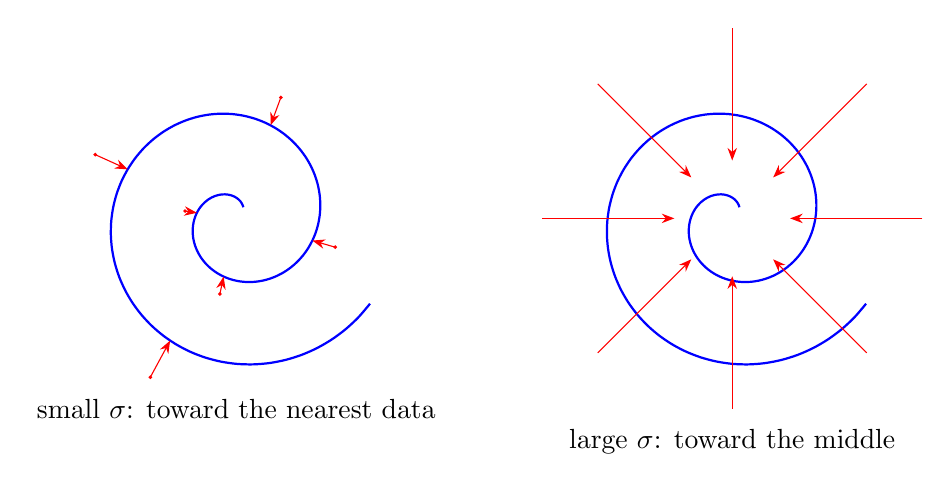
\begin{tikzpicture}[scale=2.1]
\begin{scope}
 \draw[blue,thick,domain=1:12,samples=100,smooth,variable=\t] plot ({0.08*\t*cos(\t r)},{0.08*\t*sin(\t r)});
 \foreach \t in {3,4.5,6,7.5,9,10.5}{
   \draw[-{Stealth[length=1.6mm]},red] ({1.3*0.08*\t*cos(\t r)},{1.3*0.08*\t*sin(\t r)})--({0.08*\t*cos(\t r)},{0.08*\t*sin(\t r)});
   \fill[red] ({1.3*0.08*\t*cos(\t r)},{1.3*0.08*\t*sin(\t r)}) circle (0.012);}
 \node at (0,-1.15) {small $\sigma$: toward the nearest data};
\end{scope}
\begin{scope}[xshift=3cm]
 \draw[blue,thick,domain=1:12,samples=100,smooth,variable=\t] plot ({0.08*\t*cos(\t r)},{0.08*\t*sin(\t r)});
 \foreach \a in {0,45,...,315}{\draw[-{Stealth[length=1.6mm]},red] (\a:1.15)--(\a:0.35);}
 \node at (0,-1.35) {large $\sigma$: toward the middle};
\end{scope}
\end{tikzpicture}
\caption{Original sketch of the denoiser field on the spiral (compare slide 14).}
\end{figure}

\begin{remark}[Why the loss does not reach zero]
The curve plateaus near $0.41$, not $0$. This is expected: even the best possible denoiser cannot recover $\beps$ exactly, because many $(\bx_0,\beps)$ pairs produce the same $\bx_\sigma$; the floor equals the average posterior variance of $\beps$ (Appendix~\ref{app:supp}, item~\ref{app:floor}).
\end{remark}

\subsection{The Ideal Denoiser \slides{15}}
The \textbf{ideal denoiser} minimizes the training loss; it is a function of the data set $\K$ and the noise level, and nothing else:
\begin{equation}
\beps^\ast:=\argmin_{\beps_\theta}\E_{\bx_0,\sigma,\beps}\bigl\|\beps_\theta(\bx_0+\sigma\beps,\sigma)-\beps\bigr\|^2 .
\end{equation}

\begin{theorem}[Ideal denoiser for a finite data set]\label{thm:ideal}
For a finite $\K$ (data uniformly distributed on $\K$, Gaussian noise),
\begin{equation}
\beps^\ast(\bx_\sigma,\sigma)=\frac{\sum_{\bx_0\in\K}(\bx_\sigma-\bx_0)\,\exp\!\bigl(-\|\bx_\sigma-\bx_0\|^2/2\sigma^2\bigr)}{\sigma\sum_{\bx_0\in\K}\exp\!\bigl(-\|\bx_\sigma-\bx_0\|^2/2\sigma^2\bigr)} .
\end{equation}
It is a weighted average of all data points: nearer points count more.
\end{theorem}
\begin{proof}
By the conditional-mean proposition, $\beps^\ast(\bx_\sigma,\sigma)=\E[\beps\mid\bx_\sigma]$ with $\beps=(\bx_\sigma-\bx_0)/\sigma$. By Bayes, $p(\bx_0\mid\bx_\sigma)\propto\exp(-\|\bx_\sigma-\bx_0\|^2/2\sigma^2)$ on $\K$. Taking the expectation of $(\bx_\sigma-\bx_0)/\sigma$ under these weights gives the formula.
\end{proof}

\begin{intuition}
Worked 1D example with $\K=\{-1,+1\}$, $\bx_\sigma=0.2$. For $\sigma=0.5$ the weights are $e^{-1.44/0.5}\approx0.056$ (for $-1$) and $e^{-0.64/0.5}\approx0.278$ (for $+1$), giving $\beps^\ast\approx-0.93$ and clean estimate $\hat\bx_0=0.2-0.5\cdot(-0.93)\approx0.66$: pulled toward the nearer point $+1$. For a large $\sigma=5$ the two weights are almost equal ($0.972$ vs $0.987$), $\beps^\ast\approx0.04$ and $\hat\bx_0\approx0.01$: the arrow points at the middle of the data set, exactly as in the slide's three panels ($\sigma=0.01,0.1,0.5$).
\end{intuition}

\subsection{The Smoothed Distance Function \slides{16}}
The distance to a set, $\mathrm{dist}_\K(\bx):=\inf\{\|\bx-\bx_0\|:\bx_0\in\K\}$, is not differentiable everywhere, so its gradient is hard to learn. Smoothing it by $\sigma$ fixes that.

\begin{definition}[Smoothed distance]
\begin{equation}
D_\sigma(\bx):=-\sigma^2\log\Bigl(\sum_{\bx_0\in\K}\exp\bigl(-\|\bx_0-\bx\|^2/2\sigma^2\bigr)\Bigr).
\end{equation}
(The slide denotes the smoothed squared distance by $\mathrm{dist}^2_\K(\bx,\sigma)$ and writes the identity below with a factor $\tfrac12$; with the definition as printed, $\tfrac12\mathrm{dist}^2_\K(\bx,\sigma)$ corresponds to $D_\sigma$.)
\end{definition}

\begin{proposition}[Denoiser = gradient of the smoothed distance]\label{prop:dist}
$\displaystyle \tfrac12\nabla_{\bx}\,\mathrm{dist}^2_\K(\bx,\sigma)=\nabla_{\bx}D_\sigma(\bx)=\sigma\,\beps^\ast(\bx,\sigma)$, and $\min_{\bx_0}\tfrac12\|\bx-\bx_0\|^2-\sigma^2\log|\K|\le D_\sigma(\bx)\le\min_{\bx_0}\tfrac12\|\bx-\bx_0\|^2$.
\end{proposition}
\begin{proof}
Differentiating, $\nabla D_\sigma=-\sigma^2\cdot\frac{\sum e^{-\|\bx_0-\bx\|^2/2\sigma^2}\,(-(\bx-\bx_0)/\sigma^2)}{\sum e^{-\|\bx_0-\bx\|^2/2\sigma^2}}=\frac{\sum(\bx-\bx_0)e^{\cdots}}{\sum e^{\cdots}}=\sigma\beps^\ast$ by Theorem~\ref{thm:ideal}. The bounds follow from $e^{-a_{\min}/\sigma^2}\le\sum_i e^{-a_i/\sigma^2}\le|\K|\,e^{-a_{\min}/\sigma^2}$ with $a_i=\tfrac12\|\bx-\bx_{0,i}\|^2$.
\end{proof}

\photo[3cm]{16}{the two coloured distance-field images of the cat silhouette (``On Surface'' and ``In Surface'' with the dotted arrows), with the colour bar 0--0.6}

\begin{intuition}
$\min$ has kinks where two data points are equally near; a \emph{soft}-min has none, and its slope is the vector from the weighted mean of the data to $\bx$. So the denoiser is a compass that is defined \emph{everywhere} and always points toward the data: that is what makes it a prior. Equivalently $\hat\bx_0=\bx_\sigma-\sigma\beps^\ast$ is simply the weighted mean of the data points.
\end{intuition}

\subsection{Sampling From a Diffusion Model -- Why iterative? \slides{17}}
Given a noisy $\bx_\sigma$ and its noise level, the denoiser estimates the clean point directly,
\begin{equation}
\hat\bx_0(\bx_\sigma,\sigma):=\bx_\sigma-\sigma\beps_\theta(\bx_\sigma,\sigma).
\end{equation}
A sampler walks a decreasing sequence of noise levels, taking one such estimate at each step. \textbf{DDIM} is the update
\begin{equation}\label{eq:ddim}
\bx_{t-1}=\bx_t+(\sigma_{t-1}-\sigma_t)\,\beps_\theta(\bx_t,\sigma_t).
\end{equation}

\begin{figure}[H]
\centering
\begin{tikzpicture}[font=\small]
\draw[green!50!black,thick] (0,0) .. controls (-0.6,1.3) and (1.6,2.0) .. (2.1,0.9) .. controls (2.7,-0.3) and (1,-1) .. (0,0);
\node[green!50!black] at (0.8,0.7){$\K$};
\coordinate (xt) at (7,3.8); \coordinate (x0h) at (1.3,0.1);
\coordinate (xt1) at ($(xt)!0.28!(x0h)$);
\fill (xt) circle (2pt) node[above right]{$\bx_t$};
\fill (xt1) circle (2pt) node[left]{$\bx_{t-1}$};
\fill (x0h) circle (2pt) node[below]{$\hat\bx_0^{\,t}$};
\draw[dotted,blue,thick] (xt1)--(x0h);
\draw[arr,blue] (xt)--(xt1) node[midway,above left]{$(\sigma_{t-1}-\sigma_t)\,\beps_\theta(\bx_t)$};
\end{tikzpicture}
\caption{DDIM step (redrawn from slide 17): a straight line toward the current estimate $\hat\bx_0^{\,t}$ of the data.}
\end{figure}

\begin{intuition}
One step goes only \emph{part} of the way to the current best guess, because the guess is poor while the input is very noisy; after moving, you re-evaluate the compass. The step is a straight line toward the estimate. This is the equation that depth completion reaches inside and steers (Section~\ref{sec:dc}). Algebraically the step re-noises the clean estimate to the lower level: $\bx_{t-1}=\hat\bx_0^{\,t}+\sigma_{t-1}\beps_\theta$ (Appendix~\ref{app:supp}).
\end{intuition}

\subsection{The DDIM Sampler \slides{18}}
\begin{algorithm}[DDIM sampler]\label{alg:ddim}
\texttt{for t = N, ..., 1:} \quad $\bx_{t-1}\leftarrow\bx_t+(\sigma_{t-1}-\sigma_t)\,\beps_\theta(\bx_t,\sigma_t)$; \quad \texttt{return} $\bx_0$. \\
Start from $\bx_N=\sigma_N\cdot\mathcal N(\bm0,\bm I)$.
\end{algorithm}
\begin{lstlisting}
@torch.no_grad()
def samples_ddim(model, sigmas, batchsize=1):
    xt = model.rand_input(batchsize) * sigmas[0]
    for sig, sig_prev in pairwise(sigmas):
        xt = xt - (sig - sig_prev) * model.predict_eps(xt, sig)
    return xt
\end{lstlisting}
On the toy model: \emph{fifty steps, no retraining, and the trajectory follows the field.}

\subsection{Probabilistic Sampling \slides{19}}
DDIM is deterministic: the same starting noise always gives the same sample. Adding a noise term back makes the sampler stochastic:
\begin{equation}
\bx_{t-1}=\bx_t+(\sigma_{t-1}-\sigma_t)\,\beps_\theta(\bx_t,\sigma_t)+\mu\,\bm w_t,\qquad \bm w_t\sim\mathcal N(\bm0,\bm I).
\end{equation}
(The slide writes $\sigma_{t'}$ for the next, lower level.) With $\mu=0$ this is DDIM again; as $\mu$ grows the trajectories spread, and the same input gives different samples. The slide shows $\mu=0.001,0.01,0.1$.

\begin{intuition}
$\mu$ is a ``temperature'': $\mu=0$ rolls a ball down a fixed groove, $\mu>0$ shakes the table on the way. This is the reason different seeds give different depth maps in Marigold (Section~\ref{sec:marigold}).
\end{intuition}

\subsection{Three Uses of a Prior \slides{20}}
A prior that exists as a \textbf{separate object} can be used in three ways, each a later section of the lecture.
\begin{center}\small
\begin{tabular}{@{}p{2.2cm}p{7cm}l@{}}\toprule
use & meaning & section\\\midrule
\textbf{Sample} & draw from the distribution the model represents & 3.10\\
\textbf{Condition} & train it with a side input $\bm c$, so it samples from $\mathrm p(\bx\mid\bm c)$ & 3.11\\
\textbf{Guide} & modify the state inside the sampling loop at test time, with no retraining & 3.13\\\bottomrule
\end{tabular}
\end{center}
The third is the one that turns a depth prior into a metric depth map.

\photo[3.4cm]{20}{the three panels: sampler comparison plots (Algorithm 1 vs Algorithm 2), the generated landscape (conditioning), and the super-resolution / inpainting / colorization examples (guidance)}

\subsection{The Autoencoder and Latent Diffusion \slides{21}}
Images are big, so an autoencoder compresses them first: an encoder $\mathcal E$ maps $\bx$ to a latent $\bz$, and a decoder $\mathcal D$ maps back, $\bz=\mathcal E(\bx)$, $\tilde\bx=\mathcal D(\bz)$. The autoencoder is trained \textbf{first}, then \textbf{frozen}; the diffusion model never sees pixels and you decode once, at the end. Diffusion runs on $\bz$ with the same loss:
\begin{equation}
L=\E_{\sigma,\bz_0,\beps}\Bigl[\bigl\|\beps-\beps_\theta(\bz_0+\sigma\beps,\sigma)\bigr\|^2\Bigr].
\end{equation}

\begin{figure}[H]
\centering
\resizebox{\linewidth}{!}{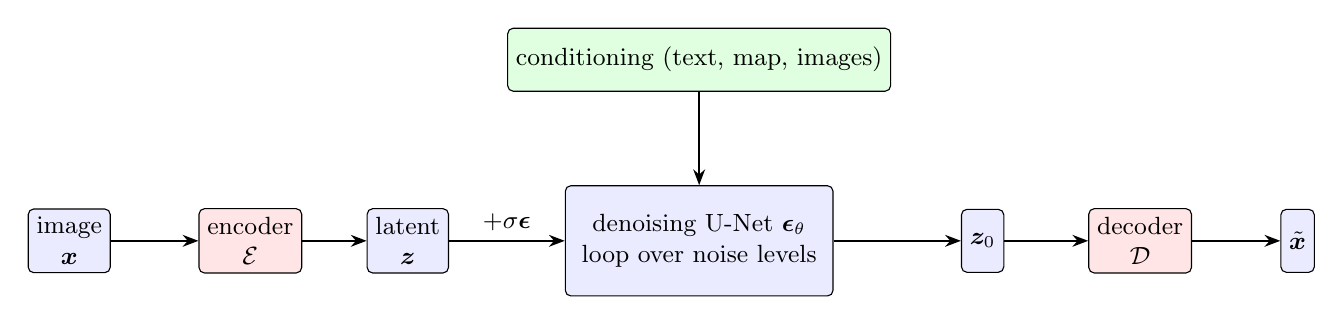
\begin{tikzpicture}[font=\small]
\node[box] (x) at (0,0){image\\$\bx$};
\node[frozen] (E) at (2.3,0){encoder\\$\mathcal E$};
\node[box] (z) at (4.3,0){latent\\$\bz$};
\node[box,minimum width=3.4cm,minimum height=1.4cm] (u) at (8,0){denoising U-Net $\beps_\theta$\\loop over noise levels};
\node[box] (z0) at (11.6,0){$\bz_0$};
\node[frozen] (D) at (13.6,0){decoder\\$\mathcal D$};
\node[box] (xt) at (15.6,0){$\tilde\bx$};
\node[box,fill=green!12] (c) at (8,2.3){conditioning (text, map, images)};
\draw[arr] (x)--(E); \draw[arr] (E)--(z); \draw[arr] (z)--node[above]{$+\sigma\beps$}(u);
\draw[arr] (u)--(z0); \draw[arr] (z0)--(D); \draw[arr] (D)--(xt); \draw[arr] (c)--(u);
\end{tikzpicture}}
\caption{Latent diffusion in outline (original, inspired by slide 21). Pink boxes are frozen autoencoder parts.}
\end{figure}

\begin{intuition}
Worked numbers: $768\times768\times3\to96\times96\times4$, i.e. $1\,769\,472$ numbers become $36\,864$: eight times smaller per side, four channels, \textbf{48 times fewer numbers}. Each of the 50 denoising steps is therefore 48 times cheaper than it would be in pixel space.
\end{intuition}

\subsection{Conditioning and Guidance \slides{22}}
\textbf{Conditioning} is a side input the network was \emph{trained with}; the model responds to it because it was trained to. \textbf{Guidance} modifies the sampling trajectory \emph{at test time}, using a criterion the network was never trained on. Sampling is a loop, and its state can be modified between steps.

\begin{figure}[H]
\centering
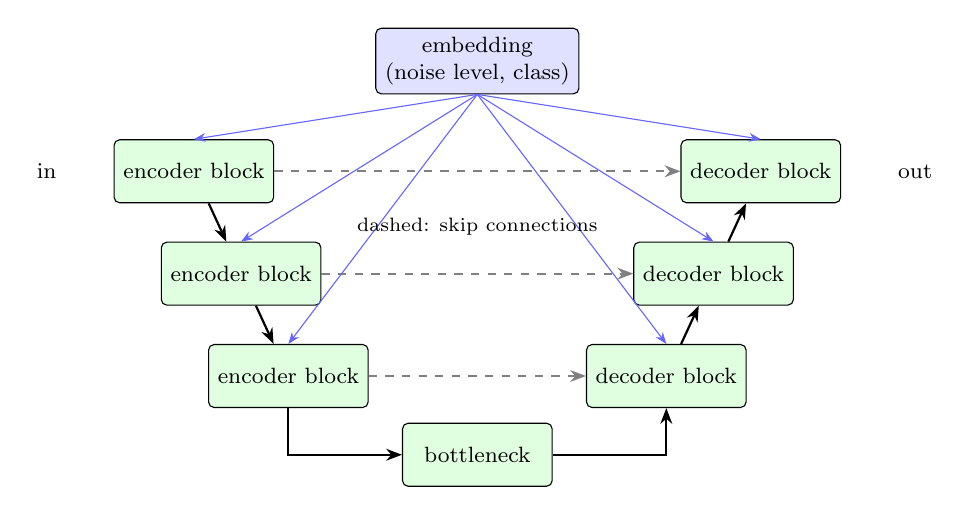
\begin{tikzpicture}[font=\footnotesize,
  blk/.style={draw,fill=green!12,minimum width=1.9cm,minimum height=0.8cm,align=center,rounded corners=2pt}]
\node[blk,fill=blue!12] (emb) at (3.6,4.4){embedding\\(noise level, class)};
\node[blk] (e1) at (0,3){encoder block};
\node[blk] (e2) at (0.6,1.7){encoder block};
\node[blk] (e3) at (1.2,0.4){encoder block};
\node[blk] (m) at (3.6,-0.6){bottleneck};
\node[blk] (d3) at (6,0.4){decoder block};
\node[blk] (d2) at (6.6,1.7){decoder block};
\node[blk] (d1) at (7.2,3){decoder block};
\draw[arr] (e1)--(e2); \draw[arr] (e2)--(e3); \draw[arr] (e3)|-(m); \draw[arr] (m)-|(d3);
\draw[arr] (d3)--(d2); \draw[arr] (d2)--(d1);
\draw[arr,dashed,gray] (e1)--(d1); \draw[arr,dashed,gray] (e2)--(d2); \draw[arr,dashed,gray] (e3)--(d3);
\foreach \n in {e1,e2,e3,d1,d2,d3}{\draw[-{Stealth[length=1.5mm]},blue!60] (emb.south)--(\n.north);}
\node[left=0.6cm of e1]{in}; \node[right=0.6cm of d1]{out};
\node[font=\scriptsize,align=center] at (3.6,2.3){dashed: skip connections};
\end{tikzpicture}
\caption{Simplified U-Net redrawn from slide 22. Each block is GroupNorm--SiLU--Conv$3{\times}3$ with the embedding injected through a Linear layer (scale and shift); attention is optional.}
\end{figure}

%=====================================================================
\section{Marigold \slides{23--31}}\label{sec:marigold}
%=====================================================================
Section 3.11: a depth estimator from an image diffusion model. Stable Diffusion's autoencoder is kept, only its denoiser is fine-tuned, and the output is a depth map rather than an image.

\subsection{The Marigold Method \slides{24}}
\emph{The argument:} a monocular estimator's knowledge of the visual world is \textbf{bounded by its training set}, while a text-to-image model trained on billions of captioned photographs has already seen it. Hence: if the cornerstone of monocular depth is a comprehensive representation of the visual world, one should be able to derive a depth estimator from a pretrained image diffusion model.

\begin{definition}[Marigold]
Take a pretrained text-to-image latent diffusion model, \textbf{freeze the VAE}, and fine-tune only the denoising U-Net so that what it denoises is a \emph{depth} latent rather than an image latent. Properties from the slide: affine-invariant monocular depth; trained on \textbf{synthetic data only}; about 2.5 days on a single consumer GPU.
\end{definition}

\photo[3.4cm]{24}{the strip of example results: photographs (beads, church, marigolds, dog, sculpture, forest, painting) with their depth maps and back-projected 3D views}

\subsection{From the Spiral to Marigold \slides{25}}
Marigold is the spiral model with one extra input; nothing in the algorithm changes.
\begin{center}\small
\begin{tabular}{@{}p{2.6cm}p{3.4cm}p{5.6cm}@{}}\toprule
 & toy model & Marigold\\\midrule
starts from & random weights & Stable Diffusion's weights\\
a data point & a 2D point & a depth latent\\
the denoiser & a small MLP & Stable Diffusion's U-Net\\
the condition & none & the image latent\\
trained on & spiral points & 74K rendered image--depth pairs\\
the sampler & DDIM & the same DDIM\\
a sample is & a point on the spiral & a depth map the RGB allows\\\bottomrule
\end{tabular}
\end{center}
The first row is the whole bet: \emph{the visual prior is already in those weights}, and fine-tuning moves what they denoise from images to depth. (Stable Diffusion indexes noise levels by a timestep $t$ and scales its input; both are fixed functions of $\sigma$, so the process is the same.)

\subsection{The Source of Affine Invariance \slides{26}}
The normalization defines the output space: the affine-invariant \emph{depth} row of the table in Part~I, not the affine-invariant \emph{disparity} row that MiDaS uses.

\begin{definition}[Percentile normalization]
With $\bm D_2$ and $\bm D_{98}$ the 2nd and 98th percentiles of the depth map $\bm D$, the training target is
\begin{equation}
\tilde{\bm D}=\Bigl(\frac{\bm D-\bm D_2}{\bm D_{98}-\bm D_2}-0.5\Bigr)\times2,\qquad\text{and metric depth is recovered as}\qquad \tilde{\bm D}_{\text{metric}}=s\tilde{\bm D}+t .
\end{equation}
\end{definition}

\begin{proposition}[Normalization removes scale and shift]
If $\bm D'=a\bm D+b$ with $a>0$, then $\tilde{\bm D}'=\tilde{\bm D}$.
\end{proposition}
\begin{proof}
Percentiles commute with increasing affine maps: $\bm D'_2=a\bm D_2+b$, $\bm D'_{98}=a\bm D_{98}+b$. Hence $(\bm D'-\bm D'_2)/(\bm D'_{98}-\bm D'_2)=a(\bm D-\bm D_2)/(a(\bm D_{98}-\bm D_2))$, the same ratio.
\end{proof}

\begin{figure}[H]
\centering
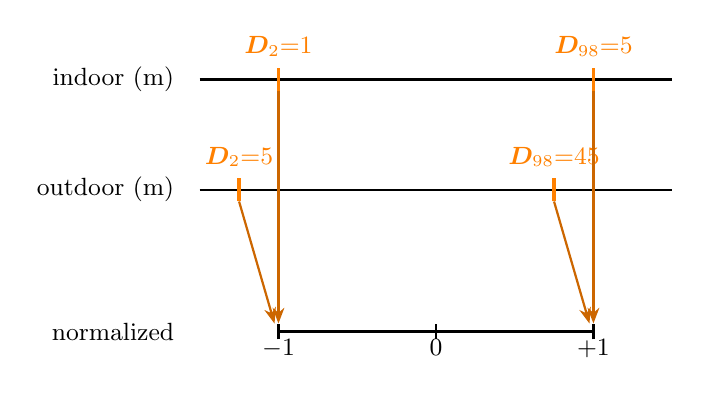
\begin{tikzpicture}[font=\small]
\draw[thick] (0,2.2)--(6,2.2); \node[anchor=east] at (-0.2,2.2){indoor (m)};
\draw[thick] (0,0.8)--(6,0.8); \node[anchor=east] at (-0.2,0.8){outdoor (m)};
\draw[thick] (1,-1)--(5,-1); \node[anchor=east] at (-0.2,-1){normalized};
\foreach \x/\l in {1/{$\bm D_2{=}1$},5/{$\bm D_{98}{=}5$}}{\draw[orange,very thick] (\x,2.05)--(\x,2.35) node[above]{\l};}
\foreach \x/\l in {0.5/{$\bm D_2{=}5$},4.5/{$\bm D_{98}{=}45$}}{\draw[orange,very thick] (\x,0.65)--(\x,0.95) node[above]{\l};}
\foreach \x/\l in {1/$-1$,3/$0$,5/$+1$}{\draw[thick] (\x,-1.1)--(\x,-0.9) node[below=2pt]{\l};}
\draw[arr,orange!80!black] (1,2.05)--(1,-0.9); \draw[arr,orange!80!black] (5,2.05)--(5,-0.9);
\draw[arr,orange!80!black] (0.5,0.65)--(0.95,-0.9); \draw[arr,orange!80!black] (4.5,0.65)--(4.95,-0.9);
\end{tikzpicture}
\caption{Original figure: an indoor map (few meters) and an outdoor map (tens of meters) land on the same $[-1,+1]$ range; each map is normalized by its \emph{own} percentiles (slide 26). The numbers are illustrative.}
\end{figure}

\begin{intuition}
Every training map is stretched to fill $[-1,+1]$, so a room and a highway look identical to the network in terms of range. \textbf{The model never sees meters and never sees a common zero, so it cannot learn them; it is constrained to predict shape.} Example: in a room with $\bm D_2=1$~m and $\bm D_{98}=5$~m, a pixel at $3$~m maps to $0$; on a street with $\bm D_2=5$~m and $\bm D_{98}=45$~m, a pixel at $25$~m also maps to $0$.
\end{intuition}

\subsection{Conditioning on the Image \slides{27}}
The denoiser takes the noisy depth latent $\bz^{(\bm D)}_\sigma$ and the image latent $\bz^{(\bm I)}$:
\begin{equation}
\beps_\theta\bigl(\bz^{(\bm D)}_\sigma,\,\bz^{(\bm I)},\,\sigma\bigr),\qquad \bz_\sigma=\mathrm{cat}\bigl(\bz^{(\bm D)}_\sigma,\bz^{(\bm I)}\bigr).
\end{equation}
The depth map is replicated to three channels and encoded by the \textbf{frozen RGB autoencoder}, whose reconstruction error on depth is negligible. \textbf{Concatenation} suits a condition that is spatially aligned with the output, pixel for pixel; cross-attention is for conditions that are not.

\begin{definition}[Four changes to the network]
(1) Concatenate the image latent and the noisy depth latent along the channels; (2) double the U-Net's input channels; (3) duplicate the first layer's weights and \textbf{halve} them, so activation magnitudes do not inflate; (4) \textbf{disable text conditioning} (original Stable Diffusion).
\end{definition}

\begin{intuition}
Why halve? Let the original first layer be $W\bz$. The new layer sees $[\bz;\bz]$ and uses $[W/2,\;W/2]$, so its output is $W\bz/2+W\bz/2=W\bz$: at the start of fine-tuning the pretrained network behaves as before. Without halving, the same input would produce $2W\bz$, twice the activations the pretrained weights expect. Since the latent has $4$ channels, the new input has $8$. Concatenation works here because the depth map and the image are aligned pixel by pixel.
\end{intuition}

\subsection{Training Marigold \slides{28}}
\begin{lstlisting}
def training_loop(loader, unet, vae, schedule, epochs):
    optimizer = torch.optim.Adam(unet.parameters())
    for _ in range(epochs):
        for image, depth in loader:                  # pairs
            optimizer.zero_grad()
            # start lock
            x0 = vae.encode(normalize(depth))        # a depth latent
            cond = vae.encode(image)                 # the condition
            # end lock
            sigma, eps = generate_train_sample(x0, schedule)
            eps_hat = unet(x0 + sigma*eps, cond, sigma)   # sees both
            loss = nn.MSELoss()(eps_hat, eps)
            loss.backward()
            optimizer.step()
\end{lstlisting}
The objective is the one from the spiral, unchanged. Only the U-Net trains; the VAE is frozen at both ends. Data: 74K rendered pairs, about 2.5 days on one consumer GPU.

\begin{figure}[H]
\centering
\resizebox{\linewidth}{!}{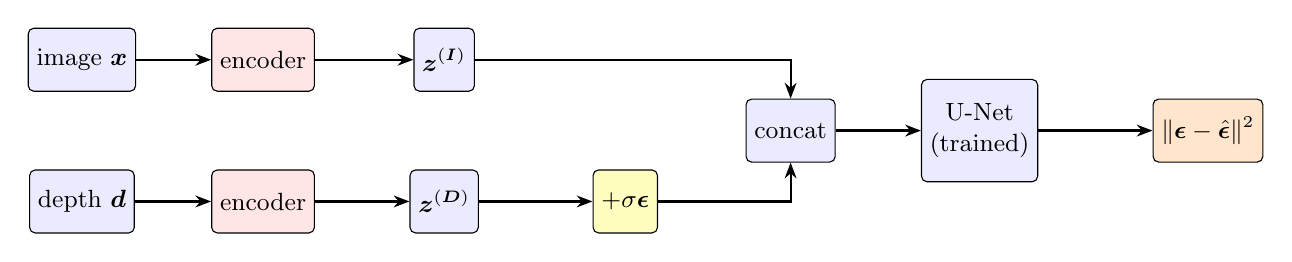
\begin{tikzpicture}[font=\small]
\node[box] (im) at (0,1.3){image $\bx$}; \node[box] (dp) at (0,-0.5){depth $\bm d$};
\node[frozen] (e1) at (2.3,1.3){encoder}; \node[frozen] (e2) at (2.3,-0.5){encoder};
\node[box] (zi) at (4.6,1.3){$\bz^{(\bm I)}$}; \node[box] (zd) at (4.6,-0.5){$\bz^{(\bm D)}$};
\node[box,fill=yellow!25] (no) at (6.9,-0.5){$+\sigma\beps$};
\node[box] (cat) at (9,0.4){concat};
\node[box,minimum height=1.3cm] (un) at (11.4,0.4){U-Net\\(trained)};
\node[box,fill=orange!20] (lo) at (14.3,0.4){$\|\beps-\hat\beps\|^2$};
\draw[arr] (im)--(e1); \draw[arr] (dp)--(e2); \draw[arr] (e1)--(zi); \draw[arr] (e2)--(zd);
\draw[arr] (zd)--(no); \draw[arr] (zi)-|(cat); \draw[arr] (no)-|(cat); \draw[arr] (cat)--(un); \draw[arr] (un)--(lo);
\end{tikzpicture}}
\caption{Marigold training (redrawn from slides 27--28). Pink: frozen. The noise $\beps$ is also fed to the loss.}
\end{figure}

\subsection{Inference \slides{29}}
\begin{algorithm}[Marigold inference, one run]
(1) Encode the image \textbf{once}; (2) initialize the depth latent $\bz_T^{(\bm D)}$ as pure Gaussian noise; (3) run the denoising loop, concatenating the image latent at \textbf{every} step; (4) decode $\bz_0^{(\bm D)}$ and average the three channels. From the paper: 50 DDIM steps.
\end{algorithm}

\begin{figure}[H]
\centering
\resizebox{\linewidth}{!}{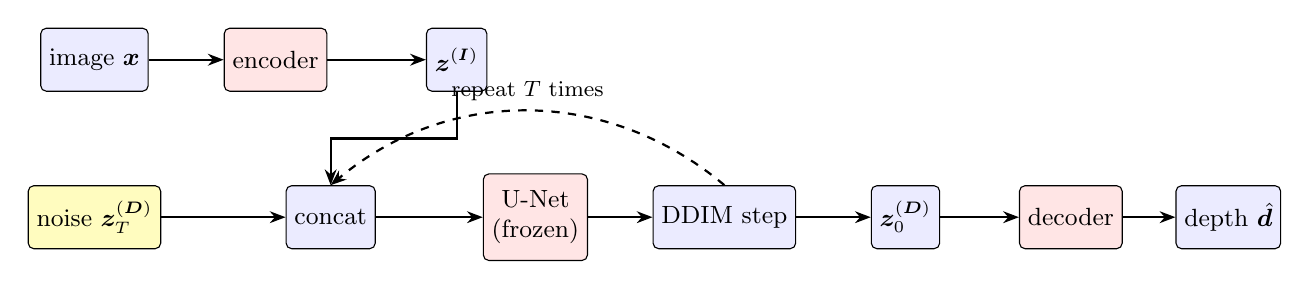
\begin{tikzpicture}[font=\small]
\node[box] (x) at (0,2){image $\bx$}; \node[frozen] (E) at (2.3,2){encoder}; \node[box] (zi) at (4.6,2){$\bz^{(\bm I)}$};
\node[box,fill=yellow!25] (n) at (0,0){noise $\bz_T^{(\bm D)}$};
\node[box] (cat) at (3,0){concat}; \node[frozen,minimum height=1.1cm] (u) at (5.6,0){U-Net\\(frozen)}; \node[box] (st) at (8,0){DDIM step};
\node[box] (z0) at (10.3,0){$\bz_0^{(\bm D)}$}; \node[frozen] (D) at (12.4,0){decoder}; \node[box] (d) at (14.4,0){depth $\hat{\bm d}$};
\draw[arr] (x)--(E); \draw[arr] (E)--(zi); \draw[arr] (zi)--++(0,-1)-|(cat);
\draw[arr] (n)--(cat); \draw[arr] (cat)--(u); \draw[arr] (u)--(st); \draw[arr] (st)--(z0); \draw[arr] (z0)--(D); \draw[arr] (D)--(d);
\draw[arr,dashed] (st.north) to[bend right=40] node[above,font=\footnotesize]{repeat $T$ times} (cat.north);
\end{tikzpicture}}
\caption{Marigold inference (redrawn from slide 29).}
\end{figure}

\subsection{Ensembling Over Samples \slides{30}}
Probabilistic sampling is why different seeds give different depth maps; Marigold runs the loop $N$ times and combines the results.
\begin{algorithm}[Ensembling]
(1) Each run is affine-invariant on its own scale, so first fit a scale and a shift per run so that the maps agree with each other (minimize the pairwise distance between the aligned maps, with a penalty that keeps the range on $[0,1]$); (2) take the pixel-wise \textbf{median}. Default $N=10$; \textbf{no ground truth is used}.
\end{algorithm}
\begin{intuition}
Ten drafts of the same drawing, each in its own unknown units. First rescale and shift each draft to line up with the others (they only agree up to $(s_i,t_i)$), then let the median vote at each pixel, which ignores outlier drafts.
\end{intuition}

\subsection{Limitations of Marigold \slides{31}}
\begin{itemize}[nosep]
 \item \textbf{No metric scale.}
 \item \textbf{No zero}: not even a common origin between two images of the same room.
 \item \textbf{Slow}: 50 denoising steps $\times$ 10 ensemble members $=500$ network evaluations per image.
 \item \textbf{It returns a sample} (non-deterministic).
\end{itemize}

%=====================================================================
\section{Back to 3D \slides{32--34}}
%=====================================================================
Section 3.12: back-projection turns a depth map into points and shows which of the unknown parameters distort the result.

\subsection{Effect of Scale and Shift Errors \slides{33}}
A depth map is a 2.5D surface: one depth per pixel, with nothing behind what is visible.

\begin{definition}[Back-projection]
A pixel with intrinsics-normalized ray $\bm r=\bm K^{-1}(u,v,1)^\top$ and depth $z$ back-projects to $\bm p=z\,\bm r$.
\end{definition}

\begin{proposition}[Affine depth error]\label{prop:affine}
If $\hat z=sz+t$, the reconstructed point is $\hat{\bm p}=(s+t/z)\,\bm p$. In particular: the \textbf{scale} $s$ multiplies the whole cloud (a similarity, so shape is preserved); the \textbf{shift} $t$ drags every point a constant depth along its own ray, a different displacement in every direction (the shape can distort).
\end{proposition}
\begin{proof}
$\hat{\bm p}=\hat z\,\bm r=(sz+t)\bm r=(s+t/z)\,z\bm r$.
\end{proof}

\begin{corollary}[Affine error in disparity]
If disparity is $\hat d=sd+t$ then $\hat z=1/\hat d$ and $\hat{\bm p}=\bm p/(s+tz)$: a \emph{projective} map of space.
\end{corollary}
\begin{proof}
$\hat z=\dfrac{1}{s/z+t}=\dfrac{z}{s+tz}$, so $\hat{\bm p}=\hat z\bm r=\bm p/(s+tz)$.
\end{proof}

\begin{figure}[H]
\centering
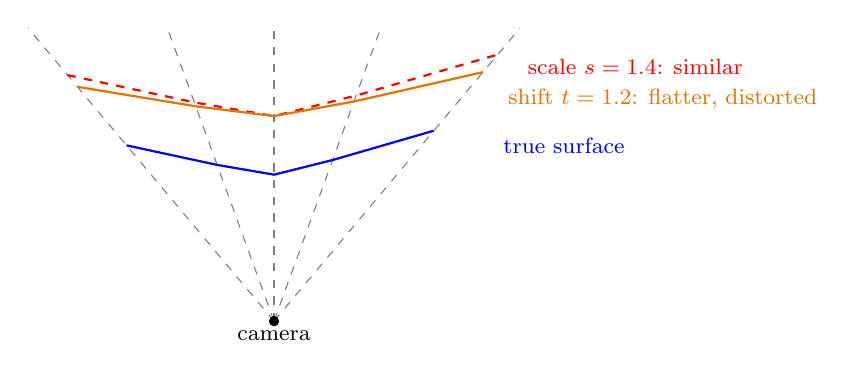
\begin{tikzpicture}[scale=0.62,font=\footnotesize]
\foreach \th in {-40,-20,0,20,40}{\draw[gray,dashed] (0,0)--({6*tan(\th)},6);}
\fill (0,0) circle (3pt) node[below]{camera};
\draw[blue,thick] (-3.02,3.6)--(-1.165,3.2)--(0,3.0)--(1.2,3.3)--(3.27,3.9);
\draw[red,thick,dashed] (-4.23,5.04)--(-1.63,4.48)--(0,4.2)--(1.68,4.62)--(4.58,5.46);
\draw[orange!90!black,thick] (-4.03,4.8)--(-1.6,4.4)--(0,4.2)--(1.64,4.5)--(4.28,5.1);
\node[blue,anchor=west] at (4.5,3.6){true surface};
\node[red,anchor=west] at (5.0,5.2){scale $s=1.4$: similar};
\node[orange!90!black,anchor=west] at (4.6,4.55){shift $t=1.2$: flatter, distorted};
\end{tikzpicture}
\caption{Original side view. A bowl-shaped surface seen along five rays. Scaling by $s$ keeps the shape (red); adding a constant depth $t$ along each ray (orange) keeps the depth differences but widens the lateral spread, so the bowl becomes flatter.}
\end{figure}

\begin{intuition}
Scale is a photocopier enlargement: bigger, same shape. Shift is pushing every point straight away from the camera by the same distance: because rays fan out, far-off directions move sideways more than the centre, so straight things bend. Example: $s=1$, $t=1$~m: a point at $z=2$ is scaled by $1+1/2=1.5$, one at $z=10$ by only $1.1$; near points are magnified more, so a wall receding from the camera is bent.
\end{intuition}

\subsection{Sources of Scale and Shift \slides{34}}
Two numbers are required, and a single image cannot supply them. Possible sources:
\begin{itemize}[nosep]
 \item a \textbf{metric-depth model}; camera-aware models narrow the generalization gap by taking the intrinsics as input (3.8);
 \item a \textbf{known baseline} at training time (3.9);
 \item a \textbf{known object size}: the apparent-size cue, which needs recognition;
 \item \textbf{known camera height plus a flat-ground assumption}: the vertical-position cue, which needs flat ground;
 \item or a \textbf{handful of real depth measurements}.
\end{itemize}

%=====================================================================
\section{Marigold-DC \slides{35--38}}\label{sec:dc}
%=====================================================================
Section 3.13: guidance from sparse depth measurements. Nothing is retrained: the denoising loop is modified at test time to move the sample toward the available measurements.

\subsection{The Depth Completion Task \slides{36}}
\begin{definition}[Depth completion]
Depth completion upgrades sparse depth measurements into dense depth maps guided by a conventional image. The sparse points come from the LiDAR returns of Part~I, structure-from-motion landmarks, or a phone's depth sensor.
\end{definition}

\photo[3.6cm]{36}{the comparison grid: ground truth, input image and the sparse guidance at high / medium / low density, with the outputs of CompletionFormer, BP-Net, VPP4DC and Marigold-DC and their RMSE labels}

\begin{center}\small
\begin{tabular}{@{}lcccc@{}}\toprule
guidance density & CompletionFormer & BP-Net & VPP4DC & Marigold-DC\\\midrule
high & 1.8 & 1.7 & 1.6 & \textbf{1.5}\\
medium & 3.7 & 2.9 & 2.0 & \textbf{1.6}\\
low & 4.8 & 3.2 & 3.3 & \textbf{2.0}\\\bottomrule
\end{tabular}\\[2pt]
RMSE values printed on slide 36 (units not stated on the slide).
\end{center}

\begin{figure}[H]
\centering
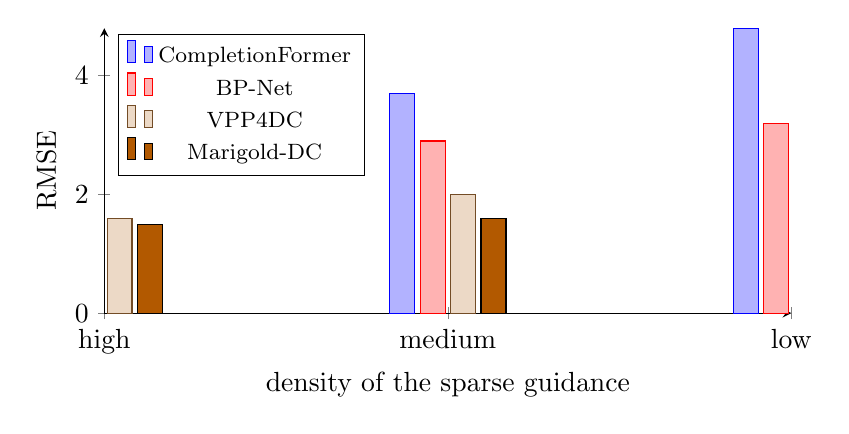
\begin{tikzpicture}
\begin{axis}[ybar,width=0.85\linewidth,height=5.2cm,bar width=9pt,ylabel={RMSE},symbolic x coords={high,medium,low},xtick=data,
  xlabel={density of the sparse guidance},ymin=0,enlarge x limits=0.25,legend style={font=\footnotesize,at={(0.02,0.98)},anchor=north west},axis lines=left]
\addplot coordinates {(high,1.8)(medium,3.7)(low,4.8)};
\addplot coordinates {(high,1.7)(medium,2.9)(low,3.2)};
\addplot coordinates {(high,1.6)(medium,2.0)(low,3.3)};
\addplot[fill=orange!70!black] coordinates {(high,1.5)(medium,1.6)(low,2.0)};
\legend{CompletionFormer,BP-Net,VPP4DC,Marigold-DC}
\end{axis}
\end{tikzpicture}
\caption{Plot of the RMSE numbers on slide 36. Baselines degrade quickly as the guidance gets sparser; Marigold-DC degrades slowly because the prior fills what the sensor did not sample.}
\end{figure}

\subsection{Steering the Loop \slides{37}}
Depth completion is reframed as \emph{image-conditional depth generation guided by sparse measurements}. It is \textbf{generation rather than regression}: the output comes from a prior. The image \textbf{conditions} the network, the sparse depth \textbf{guides} the loop, and the measurements were never part of training. Every step already walks toward the model's current estimate; a second pull is added, toward the measurements.

\begin{algorithm}[Guided step]
At every step of the loop:
(1) read the \emph{preview}, the current guess at the finished depth map, $\hat\bz_0^{\,t}=\bz_t-\sigma_t\beps_\theta$ (Tweedie formula);
(2) decode it and turn it into meters with the scale and the shift, $\hat{\bm d}^{(\mathrm m)}_t=\hat a\,\mathcal D(\hat\bz_0^{\,t})+\hat b$;
(3) compare it with the few pixels $\Omega$ that have a measurement $\bm c$, $\mathcal L=\bigl\|\hat{\bm d}^{(\mathrm m)}_t-\bm c\bigr\|_\Omega$;
(4) nudge the latent and the two scalars $(\hat a,\hat b)$ toward the measurements by gradient descent on $\mathcal L$;
(5) take the ordinary DDIM step.
\end{algorithm}

\begin{figure}[H]
\centering
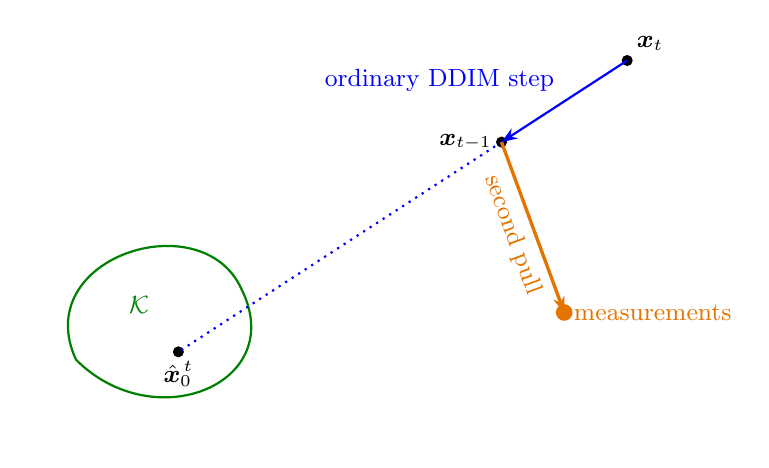
\begin{tikzpicture}[font=\small]
\draw[green!50!black,thick] (0,0) .. controls (-0.6,1.3) and (1.6,2.0) .. (2.1,0.9) .. controls (2.7,-0.3) and (1,-1) .. (0,0);
\node[green!50!black] at (0.8,0.7){$\K$};
\coordinate (xt) at (7,3.8); \coordinate (x0h) at (1.3,0.1);
\coordinate (xt1) at ($(xt)!0.28!(x0h)$);
\fill (xt) circle (2pt) node[above right]{$\bx_t$}; \fill (xt1) circle (2pt) node[left]{$\bx_{t-1}$};
\fill (x0h) circle (2pt) node[below]{$\hat\bx_0^{\,t}$};
\draw[dotted,blue,thick] (xt1)--(x0h);
\draw[arr,blue] (xt)--(xt1) node[midway,above left]{ordinary DDIM step};
\coordinate (M) at (6.2,0.6); \fill[orange!90!black] (M) circle (3pt) node[right]{measurements};
\draw[arr,orange!90!black,very thick] (xt1)--node[below,sloped]{second pull}(M);
\end{tikzpicture}
\caption{The guided step (redrawn from slide 37): DDIM step plus a second pull toward the sparse measurements.}
\end{figure}

\begin{figure}[H]
\centering
\resizebox{\linewidth}{!}{%
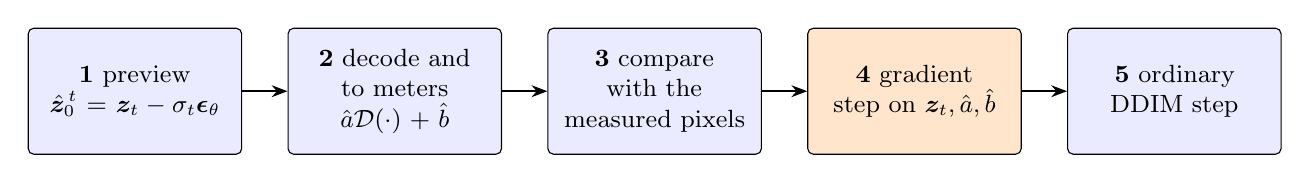
\begin{tikzpicture}[font=\small,st/.style={box,text width=2.5cm,minimum height=1.6cm}]
\node[st] (a) at (0,0){\textbf{1} preview\\$\hat\bz_0^{\,t}=\bz_t-\sigma_t\beps_\theta$};
\node[st] (b) at (3.3,0){\textbf{2} decode and to meters\\$\hat a\mathcal D(\cdot)+\hat b$};
\node[st] (c) at (6.6,0){\textbf{3} compare with the measured pixels};
\node[st,fill=orange!20] (d) at (9.9,0){\textbf{4} gradient step on $\bz_t,\hat a,\hat b$};
\node[st] (e) at (13.2,0){\textbf{5} ordinary DDIM step};
\foreach \p/\q in {a/b,b/c,c/d,d/e}{\draw[arr] (\p)--(\q);}
\end{tikzpicture}}
\caption{The five steps as a pipeline.}
\end{figure}

\subsection{Nothing Retrained \slides{38}}
Marigold gives affine-invariant depth; the sparse map gives \emph{metric} depth at a few pixels. The unknowns are the \textbf{latent}, which decides the shape, and the \textbf{scale and shift}, which decide the meters. All three are optimized, for one image, over fifty steps, and then discarded. Gradients are taken with respect to the latent and the two scalars, so \textbf{no weights change}: the U-Net and the VAE are frozen throughout.

\begin{theorem}[Zero-shot property, as claimed on the slide]
There is no depth-completion dataset, no architecture change and no new checkpoint. The method is therefore zero-shot across indoor and outdoor scenes, where the baselines ship one checkpoint per domain.
\end{theorem}

\begin{intuition}
The frozen network is a very good but unit-less sketch artist; the LiDAR points are a few tape-measure readings. At each step the sketch is bent slightly (through the latent) so that it does not contradict the readings, and the ruler (scale and shift) is adjusted until the sketch reads in meters. Because the readings are used only at test time, the same model handles a room and a street: the debts of Section~1 are paid at once, the prior supplying what the sensor cannot sample and the sensor the two numbers the prior cannot know.
\end{intuition}

\photo[3cm]{38}{the Marigold-DC diagram: goose photograph, encoder/decoder, frozen U-Net loop with the red gradient arrows, sparse map $\mathbf c$ and the resulting metric depth (the block structure is redrawn in the figures above)}

%=====================================================================
\section{Summary of Lecture 03 \slides{39--40}}
%=====================================================================
\emph{Every method in this lecture bought depth with a different resource. The last section bought it with two at once.}

\begin{center}\small
\begin{tabular}{@{}p{3.4cm}p{3.6cm}l p{4.2cm}@{}}\toprule
method & paid with & when & free parameters left\\\midrule
A laser (3.3, 3.4) & time & test & 0, but sparse\\
Stereo & a known baseline & test & 0, error grows as $z^2$\\
Structure from motion & viewpoints, no baseline & test & 1, one global scale\\
Supervised (3.7) & a prior, on sensor labels & train & 0, 1 or 2, set by the labels\\
Self-supervision (3.9) & a baseline & train & 0, for that rig\\
Marigold (3.11) & a generative prior & train & 2\\
Marigold-DC (3.13) & a prior and time & both & 0, dense, nothing retrained\\\bottomrule
\end{tabular}
\end{center}

\begin{figure}[H]
\centering
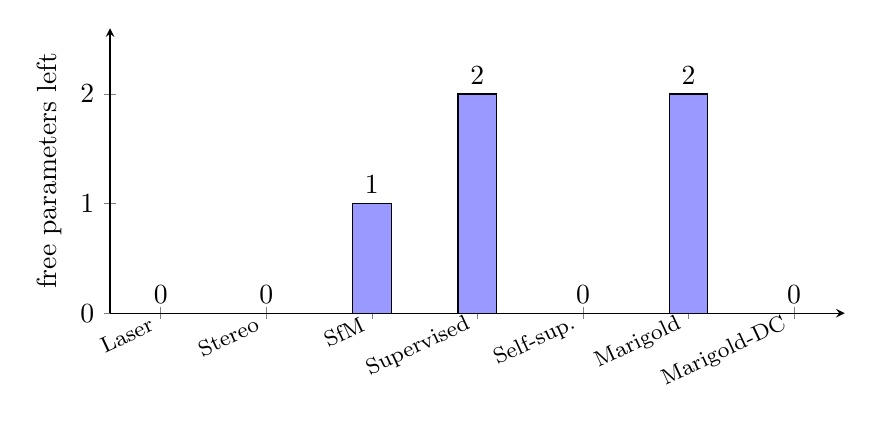
\begin{tikzpicture}
\begin{axis}[ybar,width=0.9\linewidth,height=5.2cm,bar width=14pt,symbolic x coords={Laser,Stereo,SfM,Supervised,Self-sup.,Marigold,Marigold-DC},
 xtick=data,xticklabel style={rotate=25,anchor=east,font=\footnotesize},ymin=0,ymax=2.6,ytick={0,1,2},ylabel={free parameters left},
 nodes near coords,axis lines=left,enlarge x limits=0.08]
\addplot[fill=blue!40] coordinates {(Laser,0)(Stereo,0)(SfM,1)(Supervised,2)(Self-sup.,0)(Marigold,2)(Marigold-DC,0)};
\end{axis}
\end{tikzpicture}
\caption{Free parameters left after each method (last column of the table). ``Supervised'' is drawn at its worst case: it ranges from 0 to 2 depending on the labels.}
\end{figure}

\subsection*{Key take-aways}
\begin{enumerate}[nosep]
 \item \textbf{The prior supplies what the sensor cannot sample, and the sensor supplies the two numbers the prior cannot know.}
 \item Self-supervision from stereo needs no depth labels, but the photometric loss is blind on flat and occluded pixels (hand-written priors fill the gap) and is metric only for the baseline it was trained with.
 \item A diffusion denoiser is a prior: it learns the gradient of a smoothed distance to the data, is defined everywhere, and can be sampled, conditioned, or guided; regression by contrast returns the conditional mean, which blurs depth edges.
 \item Marigold reuses Stable Diffusion's weights: frozen VAE, U-Net fine-tuned with the image latent concatenated; percentile normalization makes the output affine-invariant, so it gives shape but no meters, no common zero, and costs $50\times10=500$ evaluations.
 \item An affine error $\hat z=sz+t$ maps to $\hat{\bm p}=(s+t/z)\bm p$: scale is harmless to shape, shift distorts it. Marigold-DC fixes both by optimizing the latent, scale and shift at test time against a few metric points, with no retraining.
\end{enumerate}

\subsection*{Acknowledgments and sources \slides{41--42}}
The diffusion section (3.10) is adapted from \emph{Introduction to Diffusion}, MIT 6.S183, IAP 2026, Lecture~1, by D.~Pfrommer; parts of both halves are adapted from \emph{Depth Estimation} (Politecnico di Milano, 2024) by L.~Magri. The reference list on slide~42 (Pfrommer, Yuan, Ke et al., Rombach et al., Yang et al., Ranftl et al., Godard et al., Ho--Jain--Abbeel, Song--Meng--Ermon, Karras et al., and others) and further reading (Yuan's smalldiffusion) are given there.

%=====================================================================
\appendix
\section{Supplementary derivations (not on the slides)}\label{app:supp}
%=====================================================================
The following results are \emph{not} on the slides; they are added to justify remarks made in the main text.

\begin{proposition}[DDIM step = re-noising the clean estimate]
Equation~\eqref{eq:ddim} is equivalent to $\bx_{t-1}=\hat\bx_0^{\,t}+\sigma_{t-1}\,\beps_\theta(\bx_t,\sigma_t)$.
\end{proposition}
\begin{proof}
$\hat\bx_0^{\,t}=\bx_t-\sigma_t\beps_\theta$, hence $\bx_t=\hat\bx_0^{\,t}+\sigma_t\beps_\theta$ and $\bx_{t-1}=\bx_t+(\sigma_{t-1}-\sigma_t)\beps_\theta=\hat\bx_0^{\,t}+\sigma_{t-1}\beps_\theta$.
\end{proof}
\emph{Reading:} keep the current clean estimate and re-attach the \emph{same} predicted noise, only with the smaller amplitude $\sigma_{t-1}$.

\begin{proposition}[Irreducible floor of the training loss]\label{app:floor}
For the ideal denoiser, $L_{\text{simple}}(\beps^\ast)=\E_{\bx_\sigma,\sigma}\,\mathrm{tr}\,\mathrm{Cov}(\beps\mid\bx_\sigma)$, which is strictly positive whenever the posterior of $\bx_0$ given $\bx_\sigma$ is not a point mass.
\end{proposition}
\begin{proof}
Applying the conditional-mean decomposition of Section~3.1 with $Y=\beps$ and $f=\E[\beps\mid\bx_\sigma]$ gives $\E\|\beps-\beps^\ast\|^2=\E\,\mathrm{tr}\,\mathrm{Cov}(\beps\mid\bx_\sigma)$; and $\beps=(\bx_\sigma-\bx_0)/\sigma$, so $\mathrm{Cov}(\beps\mid\bx_\sigma)=\mathrm{Cov}(\bx_0\mid\bx_\sigma)/\sigma^2$.
\end{proof}
\emph{Reading:} this explains why the slide-14 curve stops around $0.41$ rather than $0$: the remaining loss is genuine ambiguity about which data point the noisy input came from, not an optimization failure.

\end{document}
